\section{Explainable AI and dementia}

\newcommand{\neuron}[3]{
    \node[circle, draw=black, fill=#2] (#1) at #3 {};
}


\begin{frame}{Theoretical background}
    \begin{tikzpicture}
        \node[] at (-5.25, -3.5) {};
        \node[] at (5.25, 3.5) {};

        \node[
            draw=black,
            fill=cyan!15,
            minimum height=3cm,
            minimum width=4.3cm
        ] (model) at (0, 1) {};

        \def\hsep{0.7}
        \def\vsep{0.5}
        \def\edgecolor{gray}
        \def\edgeopacity{0.5}
        \def\neuroncolour{gray}

        \only<1>{
            \node[
                anchor=south,
                font=\small
            ] at (model.north) {Artificial neural network};

            \neuron{n00}{\neuroncolour}{($ (model) + (-2 * \hsep, -2 * \vsep) $)}
            \neuron{n01}{\neuroncolour}{($ (model) + (-2 * \hsep, -\vsep) $)}
            \neuron{n02}{\neuroncolour}{($ (model) + (-2 * \hsep, 0) $)}
            \neuron{n03}{\neuroncolour}{($ (model) + (-2 * \hsep, \vsep) $)}
            \neuron{n04}{\neuroncolour}{($ (model) + (-2 * \hsep, 2 * \vsep) $)}

            \neuron{n10}{\neuroncolour}{($ (model) + (-\hsep, -1.5 * \vsep) $)}
            \neuron{n11}{\neuroncolour}{($ (model) + (-\hsep, -0.5 * \vsep) $)}
            \neuron{n12}{\neuroncolour}{($ (model) + (-\hsep, 0.5 * \vsep) $)}
            \neuron{n13}{\neuroncolour}{($ (model) + (-\hsep, 1.5 * \vsep) $)}

            \neuron{n20}{\neuroncolour}{($ (model) + (0, -\vsep) $)}
            \neuron{n21}{\neuroncolour}{(model)}
            \neuron{n22}{\neuroncolour}{($ (model) + (0, \vsep) $)}

            \neuron{n30}{\neuroncolour}{($ (model) + (\hsep, -0.5 * \vsep) $)}
            \neuron{n31}{\neuroncolour}{($ (model) + (\hsep, 0.5 * \vsep) $)}

            \neuron{n40}{\neuroncolour}{($ (model) + (2 * \hsep, 0) $)}

            \draw[-stealth, \edgecolor, opacity=\edgeopacity] (model.west) -- (n00);
            \draw[-stealth, \edgecolor, opacity=\edgeopacity] (model.west) -- (n01);
            \draw[-stealth, \edgecolor, opacity=\edgeopacity] (model.west) -- (n02);
            \draw[-stealth, \edgecolor, opacity=\edgeopacity] (model.west) -- (n03);
            \draw[-stealth, \edgecolor, opacity=\edgeopacity] (model.west) -- (n04);

            \foreach \i in {0,...,4} {
                \foreach \j in {0,...,3} {
                    \draw[\edgecolor, opacity=\edgeopacity] (n0\i) -- (n1\j);
                }
            }
            \foreach \i in {0,...,3} {
                \foreach \j in {0,...,2} {
                    \draw[\edgecolor, opacity=\edgeopacity] (n1\i) -- (n2\j);
                }
            }
            \foreach \i in {0,...,2} {
                \foreach \j in {0,...,1} {
                    \draw[\edgecolor, opacity=\edgeopacity] (n2\i) -- (n3\j);
                }
            }
            \foreach \i in {0,...,1} {
                \draw[\edgecolor, opacity=\edgeopacity] (n3\i) -- (n40);
            }

            \draw[-stealth, \edgecolor, opacity=\edgeopacity] (n40) -- (model.east);
        }
        \only<2>{
            \neuron{n00}{black!25}{($ (model) + (-2 * \hsep, -2 * \vsep) $)}
            \neuron{n01}{black!90}{($ (model) + (-2 * \hsep, -\vsep) $)}
            \neuron{n02}{black!72}{($ (model) + (-2 * \hsep, 0) $)}
            \neuron{n03}{black!99}{($ (model) + (-2 * \hsep, \vsep) $)}
            \neuron{n04}{black!10}{($ (model) + (-2 * \hsep, 2 * \vsep) $)}

            \neuron{n10}{black!55}{($ (model) + (-\hsep, -1.5 * \vsep) $)}
            \neuron{n11}{black!92}{($ (model) + (-\hsep, -0.5 * \vsep) $)}
            \neuron{n12}{black!31}{($ (model) + (-\hsep, 0.5 * \vsep) $)}
            \neuron{n13}{black!7}{($ (model) + (-\hsep, 1.5 * \vsep) $)}

            \neuron{n20}{black!50}{($ (model) + (0, -\vsep) $)}
            \neuron{n21}{black!10}{(model)}
            \neuron{n22}{black!100}{($ (model) + (0, \vsep) $)}

            \neuron{n30}{black!75}{($ (model) + (\hsep, -0.5 * \vsep) $)}
            \neuron{n31}{black!65}{($ (model) + (\hsep, 0.5 * \vsep) $)}

            \neuron{n40}{black!95}{($ (model) + (2 * \hsep, 0) $)}

            \draw[-stealth, \edgecolor, opacity=\edgeopacity] (model.west) -- (n00);
            \draw[-stealth, \edgecolor, opacity=\edgeopacity] (model.west) -- (n01);
            \draw[-stealth, \edgecolor, opacity=\edgeopacity] (model.west) -- (n02);
            \draw[-stealth, \edgecolor, opacity=\edgeopacity] (model.west) -- (n03);
            \draw[-stealth, \edgecolor, opacity=\edgeopacity] (model.west) -- (n04);

            \foreach \i in {0,...,4} {
                \foreach \j in {0,...,3} {
                    \draw[\edgecolor, opacity=\edgeopacity] (n0\i) -- (n1\j);
                }
            }
            \foreach \i in {0,...,3} {
                \foreach \j in {0,...,2} {
                    \draw[\edgecolor, opacity=\edgeopacity] (n1\i) -- (n2\j);
                }
            }
            \foreach \i in {0,...,2} {
                \foreach \j in {0,...,1} {
                    \draw[\edgecolor, opacity=\edgeopacity] (n2\i) -- (n3\j);
                }
            }
            \foreach \i in {0,...,1} {
                \draw[\edgecolor, opacity=\edgeopacity] (n3\i) -- (n40);
            }

            \draw[-stealth, \edgecolor, opacity=\edgeopacity] (n40) -- (model.east);

            \node[anchor=east, draw=black, inner sep=0pt] (input) at ($ (model.west) + (-0.77, 0) $) {
                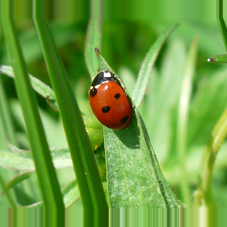
\includegraphics[width=2cm]{data/ladybug.png}
            };
            \draw[-Latex] (input) -- (model);

            \node[anchor=west] (output) at ($ (model.east) + (0.77, 0) $) {
                Ladybug
            };
            \draw[-Latex] (model) -- (output);
        }
        \only<3>{
            \neuron{n00}{red!25!black}{($ (model) + (-2 * \hsep, -2 * \vsep) $)}
            \neuron{n01}{red!90!black}{($ (model) + (-2 * \hsep, -\vsep) $)}
            \neuron{n02}{yellow!15!red}{($ (model) + (-2 * \hsep, 0) $)}
            \neuron{n03}{red!99!black}{($ (model) + (-2 * \hsep, \vsep) $)}
            \neuron{n04}{red!10!black}{($ (model) + (-2 * \hsep, 2 * \vsep) $)}

            \neuron{n10}{red!55!black}{($ (model) + (-\hsep, -1.5 * \vsep) $)}
            \neuron{n11}{yellow!20!red}{($ (model) + (-\hsep, -0.5 * \vsep) $)}
            \neuron{n12}{yellow!90!red}{($ (model) + (-\hsep, 0.5 * \vsep) $)}
            \neuron{n13}{red!7!black}{($ (model) + (-\hsep, 1.5 * \vsep) $)}

            \neuron{n20}{red!90!black}{($ (model) + (0, -\vsep) $)}
            \neuron{n21}{red!30!black}{(model)}
            \neuron{n22}{yellow!70!red}{($ (model) + (0, \vsep) $)}

            \neuron{n30}{yellow!40!red}{($ (model) + (\hsep, -0.5 * \vsep) $)}
            \neuron{n31}{red!65!black}{($ (model) + (\hsep, 0.5 * \vsep) $)}

            \neuron{n40}{red}{($ (model) + (2 * \hsep, 0) $)}

            \draw[stealth-, \edgecolor, opacity=\edgeopacity] (model.west) -- (n00);
            \draw[stealth-, \edgecolor, opacity=\edgeopacity] (model.west) -- (n01);
            \draw[stealth-, \edgecolor, opacity=\edgeopacity] (model.west) -- (n02);
            \draw[stealth-, \edgecolor, opacity=\edgeopacity] (model.west) -- (n03);
            \draw[stealth-, \edgecolor, opacity=\edgeopacity] (model.west) -- (n04);

            \foreach \i in {0,...,4} {
                \foreach \j in {0,...,3} {
                    \draw[\edgecolor, opacity=\edgeopacity] (n0\i) -- (n1\j);
                }
            }
            \foreach \i in {0,...,3} {
                \foreach \j in {0,...,2} {
                    \draw[\edgecolor, opacity=\edgeopacity] (n1\i) -- (n2\j);
                }
            }
            \foreach \i in {0,...,2} {
                \foreach \j in {0,...,1} {
                    \draw[\edgecolor, opacity=\edgeopacity] (n2\i) -- (n3\j);
                }
            }
            \foreach \i in {0,...,1} {
                \draw[\edgecolor, opacity=\edgeopacity] (n3\i) -- (n40);
            }

            \draw[stealth-, \edgecolor, opacity=\edgeopacity] (n40) -- (model.east);

            \node[anchor=east, draw=black, inner sep=0pt] (input) at ($ (model.west) + (-0.77, 0) $) {
                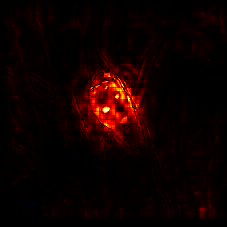
\includegraphics[width=2cm]{data/ladybug_explanation.png}
            };
            \draw[Latex-,red] (input) -- (model);

            \node[anchor=west, text=red] (output) at ($ (model.east) + (0.77, 0) $) {
                Ladybug
            };
            \draw[Latex-,red] (model) -- (output);
        }
    \end{tikzpicture}
\end{frame}

\begin{frame}{Dementia background}
    Dementia background
\end{frame}

\newcommand{\dementiadataset}{
    \begin{tikzpicture}
        \begin{axis}[
            width=\textwidth,
            height=0.4\textwidth,
            xmin=46,
            xmax=99,
            ymin=-1.6,
            ymax=1.2,
            xtick={55,60,65,70,75,80,85,90,95},
            axis lines=center,
            axis y line=none,
            clip=false
        ]
            \addplot[name path=zero, draw=none] coordinates {(47,0) (97,0)};

            \addplot[
                name path=fcases,
                draw=red,
                very thick
            ] table [
                col sep=comma,
                x=x,
                y=F-cases
            ]{data/dementia/dataset/dementia_full.csv};\label{trace:cases}
            \addplot[fill=red, opacity=0.2] fill between [of=zero and fcases];

            \addplot[
                name path=fcontrols,
                draw=blue,
                very thick
            ] table [
                col sep=comma,
                x=x,
                y=F-controls
            ]{data/dementia/dataset/dementia_full.csv};\label{trace:controls}
            \addplot[fill=blue, opacity=0.2] fill between [of=zero and fcontrols];

            \addplot[
                name path=mcases,
                draw=red,
                very thick
            ] table [
                col sep=comma,
                x=x,y
                expr=\thisrow{M-cases} * -1
            ]{data/dementia/dataset/dementia_full.csv};
            \addplot[fill=red, opacity=0.2] fill between [of=zero and mcases];

            \addplot[
                name path=mcontrols,
                draw=blue,
                very thick
            ] table [
                col sep=comma,
                x=x,
                y expr=\thisrow{M-controls} * -1
            ]{data/dementia/dataset/dementia_full.csv};
            \addplot[fill=blue, opacity=0.2] fill between [of=zero and mcontrols];

            \node[anchor=south west] at (axis cs: 46, 0.07) {\textbf{FEMALE}};
            \node[anchor=north west] at (axis cs: 46, -0.07) {\textbf{MALE}};
            \node[anchor=south, font=\footnotesize\selectfont, align=center] (n) at (axis cs: 72.5,-1.6) {n=1708};
            \node[anchor=south west,font=\footnotesize\selectfont, align=left] at ($(n.south east) + (110,0) $) {
                \ref{trace:controls} Controls\\[-0.1cm]
                \ref{trace:cases} Patients
            };
        \end{axis}
    \end{tikzpicture}
}

\newcommand{\scannersubplot}[3]{
    \nextgroupplot[
            axis lines=center,
            axis y line=none,
            xmin=46,
            xmax=99,
            ymin=-1.65,
            ymax=1.5,
            xmajorticks=false,
            axis line style={-}
        ]

            \addplot[name path=zero, draw=none] coordinates {(46, 0) (99, 0)};
            \addplot[
                name path=fcases,
                draw=red,
                very thick
            ] table [
                col sep=comma,
                x=x,
                y=F-cases
            ]{#1};
            \addplot[fill=red, opacity=0.2] fill between [of=zero and fcases];

            \addplot[
                name path=fcontrols,
                draw=blue,
                very thick
            ] table [
                col sep=comma,
                x=x,
                y=F-controls
            ]{#1};
            \addplot[fill=blue, opacity=0.2] fill between [of=zero and fcontrols];

            \addplot[
                name path=mcases,
                draw=red,
                very thick
            ] table [
                col sep=comma,
                x=x,
                y expr=\thisrow{M-cases} * -1
            ]{#1};
            \addplot[fill=red, opacity=0.2] fill between [of=zero and mcases];

            \addplot[
                name path=mcontrols,
                draw=blue,
                very thick
            ] table [
                col sep=comma,
                x=x,
                y expr=\thisrow{M-controls} * -1
            ]{#1};
            \addplot[fill=blue, opacity=0.2] fill between [of=zero and mcontrols];

            \node[anchor=south] at (axis cs: 72.5,1) {\tiny{#2}};
            \node[anchor=north] at (axis cs: 72.5,-1) {\tiny{\textbf{n=#3}}};
}

\newcommand{\dementiasubsets}{
    \begin{tikzpicture}
        \begin{groupplot}[
            group style={
                group size=5 by 2,
                horizontal sep=0.25cm,
                vertical sep=0.25cm
            },
            height=0.314\textwidth,
            width=0.314\textwidth
        ]
            \scannersubplot{data/dementia/dataset/dementia_ADNI_30T.csv}{ADNI 3.0T}{506}
            \scannersubplot{data/dementia/dataset/dementia_oasis3_30T.csv}{OASIS3 3.0T}{438}
            \scannersubplot{data/dementia/dataset/dementia_ADNI_15T.csv}{ADNI 1.5T}{290}
            \scannersubplot{data/dementia/dataset/dementia_Oslo_GE750.csv}{Oslo GE750}{226}
            \scannersubplot{data/dementia/dataset/dementia_AIBL_10.csv}{AIBL Site 1}{92}
            \scannersubplot{data/dementia/dataset/dementia_addneuromed_GE_MEDICAL_SYSTEMS.csv}{ANM GE}{74}
            \scannersubplot{data/dementia/dataset/dementia_miriad_15_T_Signa.csv}{MIRIAD}{38}
            \scannersubplot{data/dementia/dataset/dementia_AIBL_20.csv}{AIBL Site 2}{22}
            \scannersubplot{data/dementia/dataset/dementia_addneuromed_PICKER_International_Inc.csv}{ANM Picker}{12}
            \scannersubplot{data/dementia/dataset/dementia_oasis3_15T.csv}{OASIS3 1.5T}{10}
        \end{groupplot}
    \end{tikzpicture}
}


\begin{frame}{Modelling}
    \begin{tikzpicture}
        \node[] at (-5.25, -3.5) {};
        \node[] at (5.25, 3.5) {};

        \only<1>{
            \node[anchor=north] at (0, 3.5) {
                \dementiadataset
            };
            \node[] at (0, -1.5) {
                \dementiasubsets
            };
        }
        \only<2>{
            \node[] at (0, 0) {
                \cnnbox{0}
            };
        }
    \end{tikzpicture}
\end{frame}
